\documentclass[11pt, class=article, crop=false]{standalone}
\usepackage[subpreambles=true]{standalone}
\usepackage[T1]{fontenc} % for font setting
\usepackage{newtxtext, newtxmath}
\usepackage{import,
            graphicx,
            parskip,
            url,
            amsmath,
            amsthm,
            amssymb,
            wrapfig,
            fancyhdr,
            soul,
            tabularx,
            longtable}

% graphic path
\graphicspath{ {./output/} }

% side caption figure
\usepackage{sidecap}
\sidecaptionvpos{figure}{t}

% for special characters in bibliography            
\usepackage[utf8]{inputenc}
\usepackage[T1]{fontenc}

% for math
\newtheorem{proposition}{Proposition}[subsection]
\newtheorem{lemma}{Lemma}[subsection]

\theoremstyle{definition}
\newtheorem{definition}{Definition}[subsection]

% citation setup
\usepackage[euler]{textgreek}
\usepackage[sort&compress]{natbib}
\setcitestyle{square}
\setcitestyle{comma}
\bibliographystyle{pnas-new}

% caption setup
\usepackage[font={f, small}, labelfont={bf, small}]{caption}
           
% color box
\usepackage[most]{tcolorbox}
\tcbuselibrary{breakable}

% margin
\usepackage[top=2.54cm, bottom=2.54cm, left=2.54cm, right=2.54cm]{geometry}%set margin

\title{Supporting Information}
\date{} % remove date from title

\begin{document}

\renewcommand{\theequation}{S\arabic{equation}}
\renewcommand{\thetable}{S\arabic{table}}
\renewcommand{\thefigure}{S\arabic{figure}}

\maketitle

\tableofcontents

\newpage

\section{Theory}

\subsection{Preferential Prey Model}

We used the preferential prey model to generate initial food webs \citep{johnson_trophic_2014}.
The preferential prey model requires four parameters to build a food web: the number of (trophic) species $S$, the number of producer species $P$, the expected number of trophic links $N_l$, and trophic omnivory $\theta$ ($\theta > 0$).
In this model, a food web begins with $P$ primary producers, indexed as species $k = 1, 2, ..., P$.
Then, consumer species with index $k = P + 1, P + 2, ..., S$ are sequentially introduced and given their first prey $q$ randomly from those introduced earlier.
Consumer species $k$ choose, if any, additional prey $q'$ ($q' \ne q$) according to the trophic position of the first prey.

The number of additional prey, denoted as $\kappa_k$, is drawn randomly from a binomial distribution $\mbox{Bin}(a_k - 1, f_k)$, where $a_k$ is the number of species present upon the introduction of species $k$ and $f_k$ is the probability that existing species serving as prey for species $k$.
The parameter $f_k$ is assumed to be a realization of a Beta distribution:

\begin{equation}
    f_k \sim \mbox{Beta}\left(1, \frac{(S + P - 3)(S - P)}{2(N_l - S + P)} - 1\right)
\end{equation}

This parameterization ensures that the realized number of trophic links $n_l$ has the expected value of $\mathbb{E}(n_l) = N_l$ over an ensemble of food webs (Lemma \ref{lemma-beta-tilde}).

The probability of choosing prey $q'$, denoted as $Q_{q'}$, is proportional to trophic distance between $q$ and $q'$:

\begin{equation}
    Q_{q'} \propto e^{-\theta^{-1} |\tau_{q'} - \tau_q|},
\end{equation}

where $\tau_q$ is the structural trophic position of species $q$.
The trophic position of producers is one, and
consumer trophic positions are given as the average of prey trophic positions plus one:

\begin{equation}
    \tau_k = 
    \begin{cases}
    1 & ~\text{for producers}~ (k=1, 2, \ldots, P),\\
    1 + |A_{k}|^{-1} \sum_{q \in A_{k}} \tau_q & ~\text{for consumers}~ (k = P+1, P+2, \ldots, S),
    \end{cases}
    % \label{eq:def_tp}
\end{equation}

where $A_{k}$ and $|A_{k}|$ denote the set and the number of consumable prey for species $k$, respectively.

\begin{lemma}
\label{lemma-beta-tilde}
    Let $f_k$ be a random variable that follows a Beta distribution as:

    \begin{equation}
        f_k \sim \mbox{Beta}(1, \tilde{\beta}),
    \end{equation}

    where

    \begin{equation}
        \tilde{\beta} = \frac{(S + P - 3)(S - P)}{2(N_l - S + P)} - 1.
        \label{eq:beta-tilde}
    \end{equation}

    Then, the realized number of trophic links $n_l$ has the expected value of $\mathbb{E}(n_l) = N_l$.
\end{lemma}

\begin{proof}
    The realized number of trophic links $n_l$ is written as:

    \begin{align}
        \begin{split}
            n_l &= \sum_{k = P + 1}^{S}(1 + \kappa_k)\\ 
                &= (S - P) + \sum_{k = P + 1}^{S} \kappa_k.
        \end{split}
    \end{align}

    Recall that $\kappa_k \sim \mbox{Bin}(a_k - 1, f_k)$ and $f_k \sim \mbox{Beta}(1, \tilde{\beta})$.
    Then, statistical theory suggests that the variable $\kappa_k$ follows a Beta-binomial distribution as $\kappa_k \sim \mbox{Beta-binomial}(a_k - 1, 1, \tilde{\beta})$, whose expected value is $\mathbb{E}(\kappa_k) = (a_k - 1) / (1 + \tilde{\beta})$.
    Thus, we obtain

    \begin{align}
    \begin{split}
        \mathbb{E}(n_l) 
        &= (S - P) + \sum_{k = P + 1}^{S} \mathbb{E}(\kappa_k)\\
        &= (S - P) + \frac{1}{1 + \tilde{\beta}} \sum_{k = P + 1}^{S} (a_k - 1)\\
        &= (S - P) + \frac{1}{1 + \tilde{\beta}} \sum_{k = P + 1}^{S} (k - 2)~~~(\because a_k = k - 1)\\
        &= (S - P) + \frac{(S + P - 3)(S - P)}{2 (1 + \tilde{\beta})}.
    \end{split}
    \end{align}

    Using Equation \ref{eq:beta-tilde}, we yield

    \begin{equation}
        \mathbb{E}(n_l)  = N_l.
    \end{equation}
    
\end{proof}

\newpage

\subsection{Spatial Model Derivation}

\textit{Single patch dynamics} --
Our model builds upon the deterministic approximation of the continuous-time Markov process \citep{ovaskainen_asymptotically_2006}.
Let $\pi'_{ik}(t)$ be the binary random variable ($\pi'_{ik}(t) \in \{0, 1\}$) that denotes the presence (1) / absence (0) of species $k$ at patch $i$ and time $t$.
The exact dynamics can be described by a stochastic differential equation:

\begin{equation}
    \pi'_{ik}(t + dt) - \pi'_{ik}(t) = c'_{ik} (1 - \pi'_{ik}(t)) - \mu'_{ik} \pi'_{ik}(t),
    \label{eq:sde0}
\end{equation}

where $c'_{ik}$ and $\mu'_{ik}$ are time-independent Bernoulli random variables representing colonization and extinction  of species $k$ at patch $i$ with means:

\begin{align}
    \begin{split}
        \overrightarrow{c'_{ik}} &= c_{ik} dt,\\
        \overrightarrow{\mu'_{ik}} &= \mu_{ik} dt.
    \end{split}
\end{align}

The notation $\overrightarrow{\cdot}$ denotes the average over an ensemble of stochastic realizations of the temporal Markov process at patch $i$.
We rewrite Equation \ref{eq:sde0} using the means:

\begin{equation}
    d \pi'_{ik} = [c_{ik} (1 - \pi'_{ik}(t)) - \mu_{ik} \pi'_{ik}(t)]dt + d\xi_{ik}(t),
    \label{eq:sde1}
\end{equation}

where $d\xi_{ik}(t)$ is the stochastic term given by:

\begin{equation}
    d\xi_{ik}(t) = (c'_{ik} - \overrightarrow{c'_{ik}}) (1 - \pi'_{ik}(t)) - (\mu'_{ik} - \overrightarrow{\mu'_{ik}}) \pi'_{ik}(t).
\end{equation}

Here, we set $d\xi_{ik}(t) = 0$ considering the stationary state of the Markov process and focus on the deterministic component of Equation \ref{eq:sde1}, which approximates the temporal behavior of the stochastic model.
A proxy $\pi_{ik}$ ($0 \le \pi_{ik} \le 1$) is used to approximate the probability of patch $i$ being occupied ($\overrightarrow{\pi'_{ik}(t)}$), leading to the deterministic counterpart of Equation \ref{eq:sde1} expressed as:

\begin{equation}
    \frac{d \pi_{ik}}{d t} = c_{ik} (1 - \pi_{ik}) - \mu_{ik} \pi_{ik}
    \label{eq:dm0}
\end{equation}

In what follows, we use Equation \ref{eq:dm0} as the baseline model that describes the temporal evolution of occupancy probability at a single patch.

\textit{Colonization} --
We express the colonization rate $c_{ik}$ as a function of ecological and ecosystem attributes.
We define $c_{ik}$ as follows:

\begin{equation}
    c_{ik} = r_{ik} \frac{\sum_{j}^N c_{0, jk} \pi_{jk}}{N},
    \label{eq:clnz}
\end{equation}

where $r_{ik}$ is the establishment probability related to resource supply or prey availability (see below), $c_{0, jk}$ is the number of effective propagules produced by patch $j$, and $N$ is the number of patches in the ecosystem ($N = hL$, where $h$ denotes the habitat density per unit river length) .
The term $\sum_{j}^N c_{0, jk} \pi_{jk}$ represents the total number of propagules produced in the ecosystem (i.e., summed across habitat patches) after accounting for dispersal costs and species reproductive traits.
We scaled $\sum_{j}^N c_{0, jk} \pi_{ik}$ by $N$ based on the assumption that these surviving propagules are evenly allocated across habitat patches.
For simplicity, we assume that the number of propagules produced is constant over space ($c_{0, jk} = c_{0, k}$).
With notation $p_k = N^{-1}\sum_{j}^N \pi_{jk}$, this simplifying assumption yields:

\begin{equation}
     c_{ik} = r_{ik} c_{0, k} p_k
\end{equation}

The establishment probability $r_{ik}$ represents different quantities for producers and consumers:

\begin{equation}
    r_{ik} =
    \begin{cases}
    r_{0} & \text{if $k \in \text{producer}~(k = 1, 2, \ldots, P)$,}\\
    |A_k|^{-1} \sum_{q \in A_k} \pi_{iq} & \text{if $k \in \text{consumer}~(k = P + 1, P + 2, \ldots, S)$,}
    \end{cases}
    \label{eq:r-eq}
\end{equation}

where $r_0$ ($0 \le r_0 \le 1$) is the resource supply, $A_k$ is the set of prey available for species $k$ (and thus $\sum_{q  \in A_k} \pi_{iq}$ represents the expected number of prey species at patch $i$), and $|A_k|$ is the number of prey species consumable for species $k$.
This formulation assumes that resource or proportional prey availability increases species' establishment.
The resource supply $r_0$ is assumed to be constant over space.

The number of effective propagules produced by a single occupied patch $c_{0, k}$ is the product of the gross number of propagules $g_{k}$ and the survival probability during dispersal $\phi_k$.
However, we constrain $c_{0, k}$ by the number of habitat patches $N$ since $N$ is the maximum number of patches that effective propagules can colonize:

\begin{equation}
    c_{0, k} = 
    \begin{cases}
        g_k \phi_k & \text{if $g_k \phi_k < N$},\\
        N & \text{if $g_k \phi_k \ge N$}.
    \end{cases}
    \label{eq:c0-prod}
\end{equation}

The survival probability during dispersal $\phi_k$ is a function of the species-specific dispersal capability $\delta_k$ and the habitat density $h$:

\begin{equation}
    \phi_k = 1 - e^{-\delta_k h}.
    \label{eq:phi}
\end{equation}

Equation \ref{eq:phi} assumes that propagule survival during dispersal increases with increasing dispersal capability and habitat density.

\textit{Extinction} -- 
We express the extinction rate $\mu_{ik}$ as a function of disturbance, prey scarcity, and predation:

\begin{equation}
    \mu_{ik} = 
        \underbrace{\mu_{k}^{(0)} (1 + \rho u_i)}_{\text{Disturbance}} + 
        \underbrace{\mu_{k}^{(1)} \left(1 - \frac{1}{|A_k|}\sum_{q \in A_k} \pi_{iq} \right)}_{\text{Prey scarcity}} + 
        \underbrace{\mu_{k}^{(2)} \sum_{q \in \tilde{A}_k} \pi_{iq}}_{\text{Predation}},
    \label{eq:extn}
\end{equation}

where $\rho$ and $u_i$ denote the disturbance synchrony probability and the upstream river length at patch $i$, respectively, and $\tilde{A}_k$ is the set of predator species for species $k$.

The disturbance term is composed of two sources.
The first component is the stochastic disturbance occurring at the patch ($\mu_{k}^{(0)}$).
The second component is the influence of downstream disturbance cascade ($\mu_{k}^{(0)} \rho u_i$).
In rivers, any disturbance can cascade downstream as water flows downstream.
For example, the impact of environmental pollutants may be spatially extensive because they are conveyed through downstream water movement \citep{massoudieh_biogeochemical_2010}.
Similarly, flood and drought disturbances are highly correlated between up- and downstream reaches \citep{swanson_flood_1998, nakamura_disturbance_2000, sarremejane_drought_2021}, likely causing synchronized extirpation of organisms across space \citep{larsen_geography_2021}.
Our model assumes that such risks of synchronized disturbance linearly scale with the upstream river length $u_i$, allowing us to capture the essential feature of riverine systems.
The parameter $\rho$ independently controls the strength of up- and downstream synchronization.

In the second term, we assume that the extinction rate decreases with increasing species richness of available prey at patch $i$.
Specifically, the parameter $\mu_{k}^{(1)}$ denotes the extinction rate in the complete absence of consumable prey.
The extinction risk caused by the lack of prey is reduced by the factor $|A_k|^{-1} \sum_{q \in A_{k}} \pi_{iq}$, which is the ratio of the expected species richness of available prey relative to the number of consumable prey $|A_k|$.
Note that $\mu_{k}^{(1)} = 0$ for producers.

In the predation term, the extinction risk caused by predation is assumed to increase linearly with the species richness of predators at patch $i$.
The parameter $\mu_{k}^{(2)}$ defines how quickly the extinction rate increases with the expected species richness of predators $\sum_{q \in \tilde{A}_k} \pi_{iq}$.

\textit{Mean field approximation} --
With notations $\gamma_k = r_{k} c_{0, k}$ and $p_k = N^{-1} \sum_i \pi_{ik}$, we describe the temporal dynamics of the proportion of patches occupied as the spatial mean field approximation of Equation \ref{eq:dm0}, dropping subscript $i$:

\begin{equation}
    \frac{dp_k}{dt} = \gamma_k p_{k} (1 - p_{k}) - \mu_{k} p_{k},
    \label{eq:master}
\end{equation}

where

\begin{equation}
    r_{k} = 
    \begin{cases}
        r_0 & \text{if $k \in \text{producer}~(k = 1, 2, \ldots, P)$,}\\
        |A_k|^{-1} \sum_{q \in A_k} p_{q} & \text{if $k \in \text{consumer}~(k = P + 1, P + 2, \ldots, S)$,}
    \end{cases}
\end{equation}

and

\begin{equation}
    \mu_{k} = 
        \mu_{k}^{(0)} (1 + \rho \hat{u}) + 
        \mu_{k}^{(1)} \left(1 - \frac{1}{|A_k|}\sum_{q \in A_k} p_{q} \right) + 
        \mu_{k}^{(2)} \sum_{q \in \tilde{A}_k} p_{q}.
    \label{eq:extn}    
\end{equation}

The parameter $c_{0, k}$ is defined in Equations \ref{eq:c0-prod}. 
In Equation \ref{eq:extn}, we introduced the expected value of upstream river length $\hat{u}$, which can be expressed as a function of total river length $L$ and branching rate $\lambda_b$ (see Section \ref{updist} for derivation).

\newpage

\subsection{Expected Upstream River Length} \label{updist}

\begin{definition}
We derive the expected value of upstream river length, $\mathbb{E}(u)$, at a given habitat patch within a branching network characterized by total river length $L$ and branching rate $\lambda_b$.
We use the following key terms: \textit{link} and \textit{magnitude}.
A link refers to a river segment from one confluence to another or to a terminal point of the river (i.e., the upstream origin or the river mouth).
Magnitude refers to the number of exterior source links (links containing upstream terminals) flowing into a given link within the network.
The magnitude is one at an exterior source link.
Table \ref{tab:key-symbol} lists the key mathematical symbols used in this section.

\begin{SCfigure}
    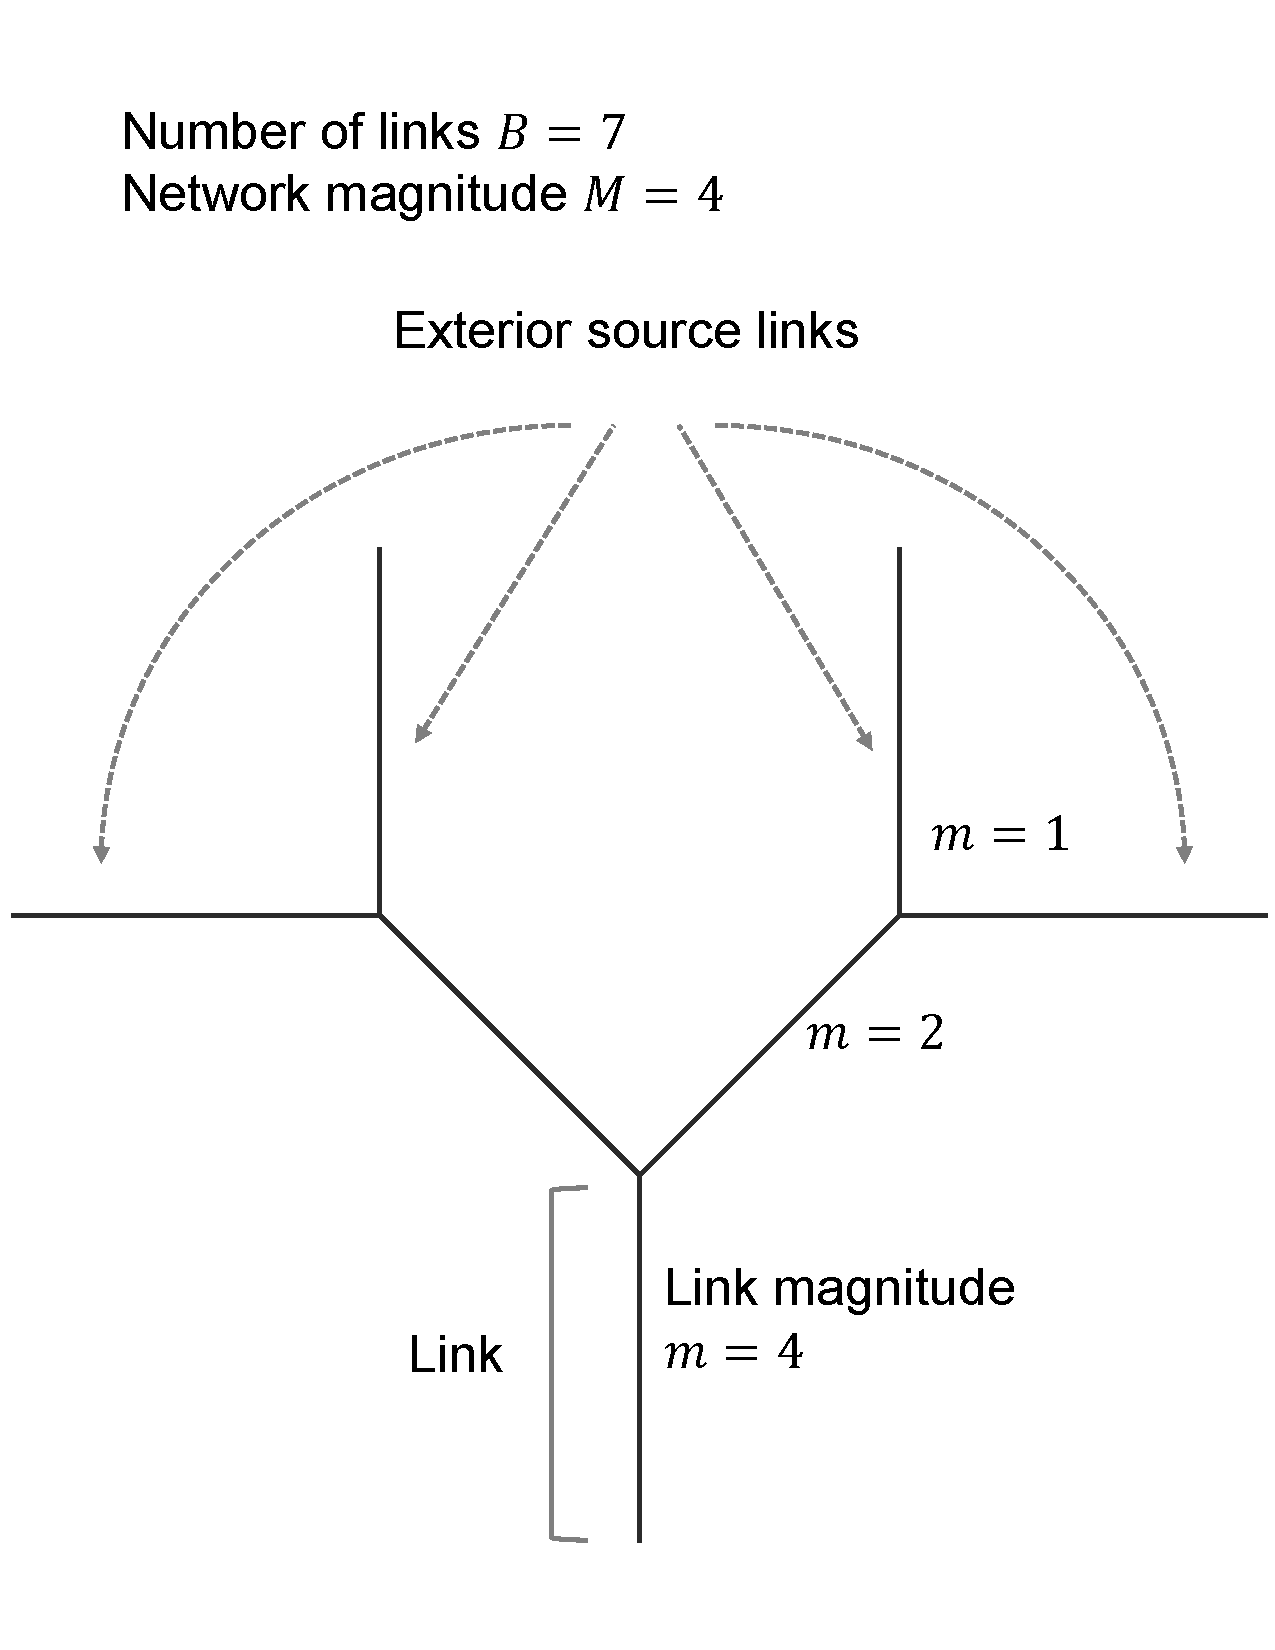
\includegraphics[width=0.4\linewidth]{output/figure_si_mag.pdf}
    \caption{text}
\end{SCfigure}

We assume that the length of individual link $s$, denoted as $l_s$, follows an exponential distribution $l_s \sim \mbox{Exp}(\lambda_b)$ with the constraint $\sum_{s = 1}^{B} l_s = L$ ($B$ denotes the number of links).
The length $l_s$ can be interpreted as the ``waiting time'' to a branching event (or termination events for upstream sources).
According to statistical theory, the number of such events within a given duration follows a Poisson distribution.
In our case, this translates into counting the number of branching events $Z$ within the ``time'' frame $L$, excluding the final branching event (since link termination occurs at $L$ regardless).
Thus, $Z \sim \mbox{Pois}(\lambda_b L)$.
The total number of links $B$ equals $Z + 1$, where adding one accounts for the final event of link termination at length $L$.
We use these assumptions in the following derivation.

\begin{table}
    \centering
    \caption{Key symbols for the derivation of expected upstream river length}
    \begin{tabularx}{\textwidth}{ll}
        \hline
        Symbol & Description\\
        \hline
        $u$ & Upstream river length at a given habitat patch.\\
        $L$ & Total river length.\\
        $\lambda_b$ & Branching rate defining the length distribution of individual links.\\
        $l$ & Individual link length. Assumed to follow $l \sim \mbox{Exp}(\lambda_b)$.\\
        $Z$ & Number of links minus one ($Z = B - 1$).\\
        \hline
    \end{tabularx}
    \label{tab:key-symbol}
\end{table}

\end{definition}

\begin{proposition}
The expected upstream river length $\mathbb{E}(u)$ at a given habitat patch within a random branching network, characterized by total river length $L$ and branching rate $\lambda_b$, can be expressed as a function of $L$ and $\lambda_b$.
\end{proposition}

\begin{proof}
The expected upstream river length, $\mathbb{E}(u)$, can be decomposed as $\mathbb{E}(u) = \mathbb{E}(u') + \mathbb{E}(l'_{s[i]})$, where $u'$ is the summed length of upstream links (excluding the link containing the habitat patch) and $l'_{s[i]}$ is the distance from the upstream link end to habitat patch $i$ in link $s$.
To calculate $\mathbb{E}(u')$ and $\mathbb{E}(l'_{s[i]})$, we condition on the number of branching events as $Z = z$ ($z \in 2\mathbb{Z}_{\ge 0}$) and the number of links as $B = b = z + 1$, whose randomness is accounted for as the final step of the proof.
We clarify this conditional assumption by denoting $\cdot ~|~ z$ in the equations.

The summed length of upstream links $u'$ is the product of the mean length of a single link $\hat{l}$ and the number of upstream links $n$.
With the known sum $\sum_{s=1}^b l_s = L$, the fraction of single link length $F_s$ (= $l_s L^{-1}$) follows a Beta distribution as $F_s ~|~ z \sim \mbox{Beta}(1, z)$ (Lemma \ref{lemma-f}), whose expected value is $\mathbb{E}(F_s~|~z) = (z + 1)^{-1}$.
Thus, we obtain an intuitive solution for the expectation of mean length as

\begin{align}
    \begin{split}
    \hat{l}~|~z = \mathbb{E}(l_s~|~z) &= L \cdot \mathbb{E}(F_s~|~z)\\
                                      &= L(z + 1)^{-1}\\
                                      &= Lb^{-1}.
    \end{split}
\end{align}

In the limit of $\lambda_b L \rightarrow \infty$, the expected value of this quantity, $\mathbb{E}(LB^{-1})$, approaches $\lambda_b^{-1}$ since $\mathbb{E}(B) = \lambda_b L + 1$.

The number of upstream links $n$ requires the consideration of its probability distribution since $n$ depends on the location in a network.
Here, our approach leverages the known properties of Shreve's topologically distinct channel networks (TDCNs) \citep{shreve_infinite_1967}, a classical framework of bifurcating river networks.
The probability of drawing a link with magnitude $m$ at random from a population of $M$-magnitude TDCNs, $\omega(m; M)$, is described as

\begin{equation}
    \omega(m; M) = \frac{1}{2m - 1} \binom{2m}{m} \binom{2(M - m)}{M - m} \binom{2M}{M}^{-1}.
\end{equation}

The notation $\binom{\cdot}{\cdot}$ and $\binom{\cdot}{\cdot}^{-1}$ denote a binomial coefficient and its inverse.
The number of upstream links $n$ has a linear relationship with link magnitude $m$ as $n = 2m - 2$ due to the bifurcating nature of TDCNs.
Using the expected value of $m$ ($\sum_{m=1}^{M} m~\omega(m; M)$; Lemma \ref{lemma-m}), we obtain

\begin{align}
    \begin{split}
    \mathbb{E}(n~|~z) 
        &= \sum_{m=1}^{M} (2m - 2) \omega(m; M)\\
        &= 2 \sum_{m=1}^{M} m~\omega(m; M) - 2\\
        &= 2 \cdot 4^{M-1} \binom{2M-1}{M}^{-1} - 2\\
        &= 2^{2M-1} \binom{2M-1}{M}^{-1} - 2.
    \end{split}
    \label{eq:n-hat}
\end{align}

TDCNs satisfy the relationship $b = 2M - 1$ because two source links must join to form a single downstream link \citep{shreve_infinite_1967, rodriguez-iturbe_fractal_2001}.
This means that $M$ is a function of $z$: $M = (b + 1) / 2 = (z + 2) / 2$.
Using this formulation, the expected value $\mathbb{E}(n~|~z)$ can be rewritten as a function of $z$:

\begin{equation}
    \mathbb{E}(n~|~z) = \hat{n}(z) = 
    2^{z + 1} \binom{z + 1}{\frac{z + 2}{2}}^{-1} - 2.
\end{equation}

In sum, we obtain $\mathbb{E}(u' ~|~ z)$ as

\begin{align}
    \begin{split}
        \mathbb{E}(u' ~|~ z) 
        &= \hat{l} \cdot \mathbb{E}(n ~|~ z)\\
        &= \frac{L \hat{n}(z)}{z + 1}.
    \end{split}
\end{align}

Note that we used $\mathbb{E}(u' ~|~ z)  = \hat{l} \cdot \mathbb{E}(n ~|~ z)$ in light of the lack of covariance between $\hat{l}$ and $n$.

The expected distance $\mathbb{E}(l'_{s[i]}~|~z)$ is calculated as follows.
Assuming that habitat patches are randomly distributed along the river (i.e., Poisson process), the distance to habitat patch $i$ in link $s$, $l'_{s[i]}$, follows a uniform distribution, i.e.,  $\Pr(l'_{s[i]}~|~z, l_s) = \mbox{Unif}(0, l_s)$.
Thus, the conditional expectation of the distance is

\begin{equation}
    \mathbb{E}(l'_{s[i]}~|~z, l_s) = \frac{l_s}{2}.
\end{equation}

% Now, we derive the expected distance to a habitat in a focal link $\mathbb{E}(l'_{s[i]}~|~z)$.
Recall that the conditional probability of the distance to a given patch is $\Pr(l'_{s[i]}~|~z)= \int \Pr(l'_{s[i]}~|~z, l_s) \Pr(l_s~|~z)d l_s$, and that the expected length of link $s$ is $\mathbb{E}(l_s~|~z) = L(z+1)^{-1}$.
Then, we obtain 

\begin{align}
    \begin{split}
        \mathbb{E}(l'_{s[i]}~|~z)
        &= \int l'_{s[i]} \Pr(l'_{s[i]}~|~z) dl'_{s[i]}\\
        &= \iint l'_{s[i]} \Pr(l'_{s[i]}~|~z, l_s) \Pr(l_s~|~z) dl'_{s[i]} dl_s \\
        &= \int \frac{l_s}{2} \Pr(l_s~|~z) dl_s \\
        &= \frac{L}{2(z + 1)}.
    \end{split}
\end{align}

Summing $\mathbb{E}(u' ~|~ z)$ and $\mathbb{E}(l'_{s[i]}~|~z)$ for a network with a given value of $z$ yields

\begin{align}
    \begin{split}
        \mathbb{E}(u ~|~ z) 
        &= \mathbb{E}(u' ~|~ z) + \mathbb{E}(l'_{s[i]}~|~z)\\
        &= \frac{L}{z+1} \left[ \hat{n}(z) + \frac{1}{2} \right].
    \end{split}
    \label{eq:cu}
\end{align}

Lastly, we account for the probabilistic nature of the random variable $Z$ by summing $z$ out from Equation \ref{eq:cu}.
In a bifurcating network, $Z$ must be even so that the total number of links $B$ is odd.
As such, we must consider a truncated Poisson distribution for $Z$ with zero probabilities for odd integers, denoted as $f'_{\text{pois}}(z; L, \lambda_b)$:

\begin{align}
    \begin{split}
    f'_{\text{pois}}(z; L, \lambda_b) 
    &= \frac{f_{\text{pois}}(z; L, \lambda_b)}{\Pr(Z \in 2\mathbb{Z}_{\ge 0})} \cdot \frac{1 + (-1)^{z}}{2}\\
    &= f_{\text{pois}}(z; L, \lambda_b) \cdot \frac{1 + (-1)^{z}}{1 + e^{-2\lambda_b L}},
    \end{split}
    \label{eq:tpois}
\end{align}

where $f_{\text{pois}}(z; L, \lambda_b)$ is the probability mass function of a Poisson distribution defined as

\begin{equation}
    f_{\text{pois}}(z; L, \lambda_b) = \Pr(Z = z) = \frac{(\lambda_b L)^{z} e^{-\lambda_b L}}{z!},
\end{equation}

and $\Pr(Z \in 2\mathbb{Z}_{\ge 0}) = 2^{-1}(1 + e^{- 2 \lambda_b L})$ (Lemma \ref{lemma-pois}). 
% In Equation \ref{eq:tpois}, $f_{\text{pois}}(z; L, \lambda_b)$ is divided by the probability of $Z$ taking even integers $\Pr(Z = \text{even})$ so that $\sum_{z=0}^{\infty} f'_{\text{pois}}(z; L, \lambda_b) = 1$.
Following the definition of expected value, we obtain $\mathbb{E}(u)$ as a function of $L$ and $\lambda_b$:

\begin{align}
    \begin{split}
        \mathbb{E}(u) = \hat{u}(L, \lambda_b) 
                    &= \sum_{z \in 2\mathbb{Z}_{\ge 0}} \left[ \frac{L}{z + 1} \left(\hat{n}(z) + \frac{1}{2}\right) f'_{\text{pois}}(z; L, \lambda_b) \right]\\
                    &= L \sum_{z \in 2\mathbb{Z}_{\ge 0}} \left[ \frac{\hat{n}(z)}{z + 1} f'_{\text{pois}}(z; L, \lambda_b)\right] + 
                    \frac{1 - e^{-2 \lambda_b L}}{2 \lambda_b (1 + e^{-2 \lambda_b L})}.
    \end{split}
\end{align}
\end{proof}

\newpage

\begin{lemma}
\label{lemma-f}
Let link length $l_1, l_2, \ldots, l_b$ be independent random variables that follow $\mbox{Exp}(\lambda_b)$.
If the total length is given as $\sum_{s=1}^b l_s = L$, the fraction of single link length $F_s = l_s L^{-1}$ follows a Beta distribution $\mbox{Beta}(1, z)$.
\end{lemma}

\begin{proof}
An exponential distribution $\mbox{Exp}(\lambda_b)$ is a special case of Gamma distribution, i.e., $\mbox{Ga}(1, \lambda_b)$.
Thus, $l_1, l_2, \ldots, l_b$  follow $\mbox{Ga}(1, \lambda_b)$.
Let us denote $X_1 = l_s$, $X_2 = \sum_{s'}^b l_{s'}$ ($s' \in \{1,2, \ldots, b\} \setminus \{s\}$), and $X_1 + X_2 = Y$.
Given the reproductive property of Gamma distribution, $X_2 \sim \mbox{Ga}(z, \lambda_b)$ and $Y \sim \mbox{Ga}(z + 1, \lambda_b)$.
The conditional probability density of $X_1 = x$ ($0 \le x \le L$) given $Y = L$, denoted as $f_{X_1}(X_1 = x~|~Y = L)$, is

\begin{align}
    \begin{split}
        f_{X_1}(X_1 = x~|~Y = L)
        &= \frac{f_{X_1}(X_1 = x~|~Y = L) f_{X_2}(X_2 = L - x~|~Y = L)}{f_Y(Y = L)}\\
        &= 
        \left[
        \frac{\lambda_b^{1 + z}}{\Gamma(1) \Gamma(z)} (L - x)^{z - 1} e^{-\lambda_b L}
        \right]
        \left[
        \frac{\lambda_b^{1 + z}}{\Gamma(1 + z)} L^{z} e^{-\lambda_b L}
        \right]^{-1}\\
        &= \frac{\Gamma(1 + z)}{\Gamma(1) \Gamma(z) L^{z}} (L - x)^{z - 1}.
    \end{split}
    \label{eq:beta}
\end{align}

Equation \ref{eq:beta} indicates that $f_{X_1}(X_1 = x~|~Y = 1)$ is the probability density function of $\mbox{Beta}(1, z)$.
Thus, we obtain

\begin{equation}
    F_s=\frac{l_s}{L} \sim \mbox{Beta} (1, z).
\end{equation}

\end{proof}

\begin{lemma}
\label{lemma-m}
Let $\omega(m; M)$ be a probability mass function defined as

\begin{equation}
    \omega(m; M) = \frac{1}{2m - 1} \binom{2m}{m} \binom{2(M - m)}{M - m} \binom{2M}{M}^{-1}.
\end{equation}

Then, the expected value of $m$ is given by

\begin{equation}
    \mathbb{E}(m; M) = \sum_{m = 1}^M m~\omega(m; M) = 4^{M-1} \binom{2M-1}{M}^{-1}.
\end{equation}
\end{lemma}

\begin{proof}
We begin by reorganizing the probability mass function

\begin{equation}
    \omega(m; M) = \frac{(2M - 2m - 1) M}{(M - m)(2M - 1)} \omega(m; M - 1).
\end{equation}

From this, we can express

\begin{equation}
    (M - m) \omega(m; M) = \frac{(2M - 2m - 1) M}{2M - 1} \omega(m; M - 1).
\end{equation}

Summing over all $m$, we get

\begin{equation}
    \sum_{m = 1}^{M - 1} (M - m) \omega(m; M)
    = \sum_{m = 1}^{M} (M - m) \omega(m; M)
    = \frac{M}{2M - 1} \sum_{m = 1}^{M - 1} (2M - 2m - 1) \omega(m; M - 1).
\end{equation}

Using the fact that $\sum_{m = 1}^{M} \omega(m; M) = 1$, the equation above leads to the following recurrence relation for the expected value:

\begin{equation}
    \mathbb{E}(m; M) = \frac{2M}{2M - 1} \mathbb{E}(m; M - 1).
\end{equation}

Considering $\mathbb{E}(m; M = 1) = 1$, we can recursively calculate the expected value:

\begin{equation}
    \mathbb{E}(m; M) = \frac{2M}{2M - 1} \cdot \frac{2M - 2}{2M - 3} \cdot \ldots \cdot \frac{4}{3} \cdot \mathbb{E}(m; 1) = 4^{M - 1} \frac{M!(M - 1)!}{(2M - 1)!}.
\end{equation}

Thus, we conclude

\begin{equation}
    \mathbb{E}(m; M) = 4^{M - 1} \binom{2M - 1}{M}^{-1}.
\end{equation}
\end{proof}

Yutaka Osada and Ryosuke Iritani contributed this Lemma.

\begin{lemma}
\label{lemma-pois}
Let $f_{\text{pois}}(y; \lambda) = \Pr(Y = y)$ be the probability mass function of a Poisson distribution.
Then, $\Pr(Y \in 2\mathbb{Z}_{\ge 0}) = 2^{-1}(1 + e^{- 2 \lambda})$.
\end{lemma}
\begin{proof}
\begin{align}
    \begin{split}
        \Pr(Y \in 2\mathbb{Z}_{\ge 0}) 
        &= \sum_{y = 0}^{\infty} \left[ \frac{\lambda^{y} e^{-\lambda}}{y!} \cdot \frac{1 + (-1)^{y}}{2} \right]\\
        &= \frac{e^{-\lambda}}{2} \left[ \sum_{y = 0}^{\infty} \frac{\lambda^{y}}{y!} + \sum_{y = 0}^{\infty} \frac{(-\lambda)^{y}}{y!}\right]\\
        &= \frac{e^{-\lambda}}{2} (e^{\lambda} + e^{-\lambda}) ~ (\because \text{Maclaurin series expansion of exponential function})\\
        &= \frac{1 + e^{- 2 \lambda}}{2}.
    \end{split}
\end{align}
\end{proof}

\newpage

\subsection{Uniqueness of Stable Equilibrium}
 
\begin{proposition}
Under the condition that $\mu_k^{(2)} = 0$, the system given by Equation \ref{eq:master} has a unique locally stable equilibrium.
\end{proposition}

\begin{proof}
The fraction of patches occupied by species $k$ at equilibrium is written as follows:

\begin{align}
    \frac{dp_k}{dt} = 0 \Leftrightarrow p_k = 
         0 ~\text{or}~
         p_{k}^{*},
\end{align}

where $p_{k}^{*} = 1 - \mu_k / \gamma_k$.
Note that $p_{k}^{*} <0 \Leftrightarrow \gamma_k-\mu_k<0$ is biologically meaningless.

Under the preferential prey model, species $k$ may consume a subset of species $1,2,\ldots, k-1$ but not $k+1, k+2, \ldots, S$ because the food web is acyclic (see Methods in the main text).
This implies that $\mu_k$ and $\gamma_k$ depend on at least one of $p_1, p_2, \ldots, p_{k-1}$, but are independent of $p_{k+1}, p_{k+2}, \ldots, p_{S}$.

The Jacobian matrix of Equation \ref{eq:master}, denoted as $J$, is then lower-triangular.
The characteristic equation of this Jacobian matrix at equilibrium is given as:

\begin{align}
    \begin{split}
        &|\lambda I - J| = 0\\
        \Leftrightarrow 
        &\prod_{k=1}^{S}(\lambda -J_{kk})=0\\
        \Leftrightarrow
        &\lambda = J_{kk}~ \forall k,
    \end{split}
\end{align}

where $I$ and $\lambda$ are the identity matrix and the eigenvalue, respectively, and 

\begin{align}
    \begin{split}
        J_{kk}  &= \gamma_k(1-2p_k)-\mu_k \\
                &=\left\{
                       \begin{array}{cl}
                       \mu_k - \gamma_k& \text{if}~ p_k=p_k^*\\
                       \gamma_k - \mu_k& \text{if}~ p_k=0.
                       \end{array}
                   \right.
    \end{split}
\end{align}

An equilibrium is locally stable if and only if all eigenvalues $\lambda$ are negative. Therefore, a focal equilibrium is locally stable if and only if

\begin{align}
    \lambda < 0 &\Leftrightarrow 
    \left\{
    \begin{array}{cc}
         \mu_k - \gamma_k < 0   &\text{if}~ p_k = p_k^*\\
         \gamma_k - \mu_k < 0   &\text{if}~ p_k = 0.
    \end{array}
    \right.
    \label{eq:eigenvalue}
\end{align}

Equation \ref{eq:eigenvalue} indicates that $\mu_k - \gamma_k < 0$ for persistent species ($p_k = p_k^*>0$) and $\gamma_k - \mu_k < 0$ for extinct species ($p_k=0$) at a stable equilibrium.

Now, we demonstrate the uniqueness of the stable equilibrium, despite the system having multiple equilibria due to the various permutational combinations of persistent and extinct species.
For producer species ($k=1,2,\ldots, P$), $\gamma_k-\mu_k$ is constant as follows:

\begin{align}
    \gamma_k-\mu_k = r_0 c_{0, k} - \mu_{k}^{(0)} (1 + \rho \hat{u}).
\end{align}

This indicates the unique combination of the persistent and extinct producers at a stable equilibrium.
For consumer species ($k = P+1, P+2,\ldots, S$), $\gamma_k-\mu_k$ depends on $p_1, p_2, \ldots, p_{k-1}$ as follows:

\begin{align}
    \gamma_k-\mu_k = \frac{\left(c_{0, k}+\mu_{k}^{(1)}\right)}{|A_k|}\sum_{q \in A_k} p_q
- \mu_{k}^{(0)} (1 + \rho \hat{u})-\mu_{k}^{(1)} ,
\end{align}

where $A_k$ is the set of consumable prey for species $k$.

Recall that $A_k$ does not include species $q = k, k+1, \ldots, S$ due to the acyclic nature of the food web.
For species $k = P+1$, the value of $\mu_k-\gamma_k$ at a stable equilibrium is unique because the producer's occupancy at a stable equilibrium ($p_1, p_2, \ldots, p_P$) is unique (i.e., $\sum_{q \in A_k} p_q$ is unique).
In other words, the persistence state of the producer species at a stable equilibrium uniquely determines the state of species $k = P+1$ at a stable equilibrium.
This logic recursively applies to species $k=P+2. \ldots, S$.
Therefore, the system given by Equation \ref{eq:master} has a unique stable equilibrium.
\end{proof}

\newpage

\subsection{No Cascade Model}

To investigate how disturbance cascades alter the qualitative predictions, we developed a model without disturbance cascades.
This ``no cascade'' model is identical to the one presented in the main text, except for the extinction rate $\mu_k$, which was modified as follows:

\begin{equation}
    \mu_{k} = 
        \underbrace{\mu_{k}^{(0)} o}_{\text{Disturbance}} + 
        \underbrace{\mu_{k}^{(1)} \left(1 - \frac{1}{|A_k|}\sum_{q \in A_k} p_{q} \right)}_{\text{Prey scarcity}} + 
        \underbrace{\mu_{k}^{(2)} \sum_{q \in \tilde{A}_k} p_{q}}_{\text{Predation}}.
\end{equation}

Here, $o$ is a constant used to ensure that the disturbance rate is comparable to the rates explored in the model with spatial disturbance cascades.
We assumed $o = 1 + \rho \hat{u}~(L = 55, \lambda_b = 0.55)$, and other parameter values are specified as described in Table 1 (analytical).
Model predictions are displayed in Figure \ref{fig:no-cascade}.

\begin{figure}
\centering
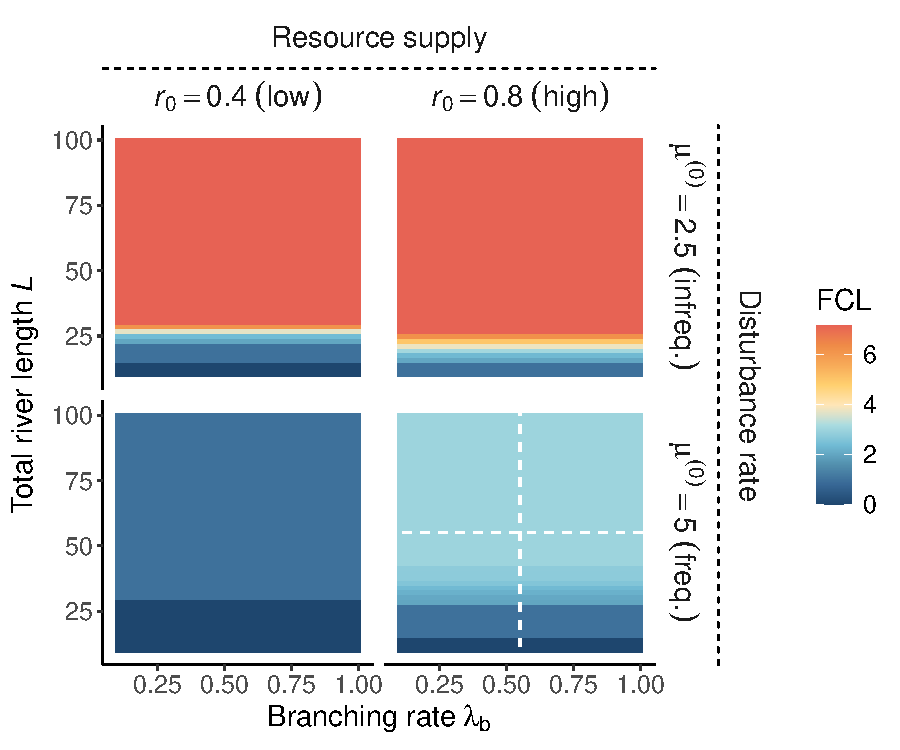
\includegraphics[width=0.75\textwidth]{fig_theo_rho0.pdf}
\caption{Analytical prediction with no disturbance cascade. Heatmaps of
FCL are expressed as a function of ecosystem size (river length, \(L\))
and complexity (branching rate, \(\lambda_b\)), with rows and columns
reflecting different disturbance and resource supply regimes. Each cell
represents the average FCL of 20 food webs. White dashed lines indicate
specific scenarios, explored in Figure 2B and 2C in the main text.
Additional parameter values are provided in Table 1.}
\label{fig:no-cascade}
\end{figure}

\newpage

\subsection{Numerical Analysis}

We performed a numerical sensitivity analysis to validate the robustness of analytical predictions in broader ecological contexts.
Specifically, we allowed additional variations in prey and predation influences ($\mu^{(1)}$ and $\mu^{(2)}$), propagule size ($g_0$), synchrony probability ($\rho$), and omnivory level ($\theta$), resulting in 128 simulation scenarios (Table \ref{tab:parms-num}).

In each simulation scenario, we considered 20 values of total river length $L$ and branching rate $\lambda_b$ within the value ranges identical to the main analysis (see Methods).
In light of the broader parameter space and the computational costs of numerical analysis, we simulated five replicas of food webs through the procedure described in the main text.
An absorbing condition for this numerical analysis is $10^{-5}$, meaning that species with $p_k < 10^{-5}$ are removed (extinct) from the simulation run.
This numerical exploration results in $5 \times 128~\times~20^2 = 256,000$ runs.
Model predictions are displayed in Figures \ref{fig:fig-num1} -- \ref{fig:fig-num8}.

\begin{table}[ht]
\centering
\caption{Parameter descriptions and values used for numerical predictions.} 
\label{tab:parms-num}
\begingroup\small
\begin{tabularx}{\textwidth}{lll}
  \hline
Symbol & Description & Value \\ 
  \hline
$r_0$ & Resource supply [-] & 0.25, 0.50 \\ 
  $\omega$ & Effect of stream size on the establishment of basal species [per unit river length] & 0.01 \\ 
  $g_0$ & Number of propagules for producers [-] & 75, 150 \\ 
  $\delta_0$ & Dispersal capability for producers [unit river length] & 0.50 \\ 
  $h$ & Habitat density [per unit river length] & 2.50 \\ 
  $\mu^{(0)}$ & Disturbance-induced extinction rate [per unit time] & 2.50, 5.00 \\ 
  $\mu^{(1)}$ & Maximum prey-induced extinction rate [per unit time] & 2.50, 5.00 \\ 
  $\mu^{(2)}$ & Predator-induced extinction rate [per unit time] & 1.25, 2.50 \\ 
  $\rho$ & Synchrony probability [-] & 0.25, 0.50 \\ 
  $\psi$ & Scaling exponent for propagule and dispersal parameters [per unit ln trophic position] & 0.50 \\ 
  $\theta$ & Degree of omnivory [per unit trophic position] & 0.25, 0.50 \\ 
   \hline
\end{tabularx}
\endgroup
\end{table}


\newpage

\begin{figure}
\centering
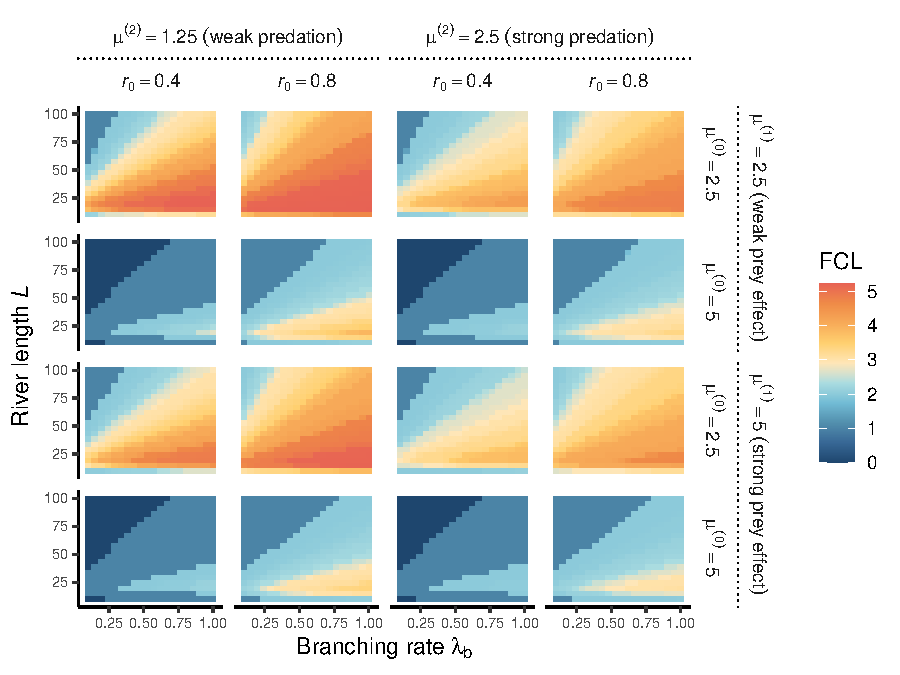
\includegraphics{../output/fig_theo_rho025_g75_theta025.pdf}
\caption{\label{fig:fig-num1}Numerical prediction with low propagule
\(g_0 = 75\), low synchrony \(\rho = 0.25\), and weak omnivory
\(\theta = 0.25\). Heatmaps of FCL are expressed as a function of
ecosystem size (river length, \(L\)) and complexity (branching rate,
\(\lambda_b\)), with rows and columns displaying different combinations
of resource supply (\(r_0\)), disturbance regime (\(\mu^{(0)}\)), prey
effect (\(\mu^{(1)}\)), and predation effect (\(\mu^{(2)}\)). Each cell
represents the average FCL of five food webs. Additional parameter
values are: habitat density \(h=2.5\), dispersal capability
\(\delta_0=0.5\), and scaling exponent \(\psi=0.5\).}
\end{figure}

\newpage

\begin{figure}
\centering
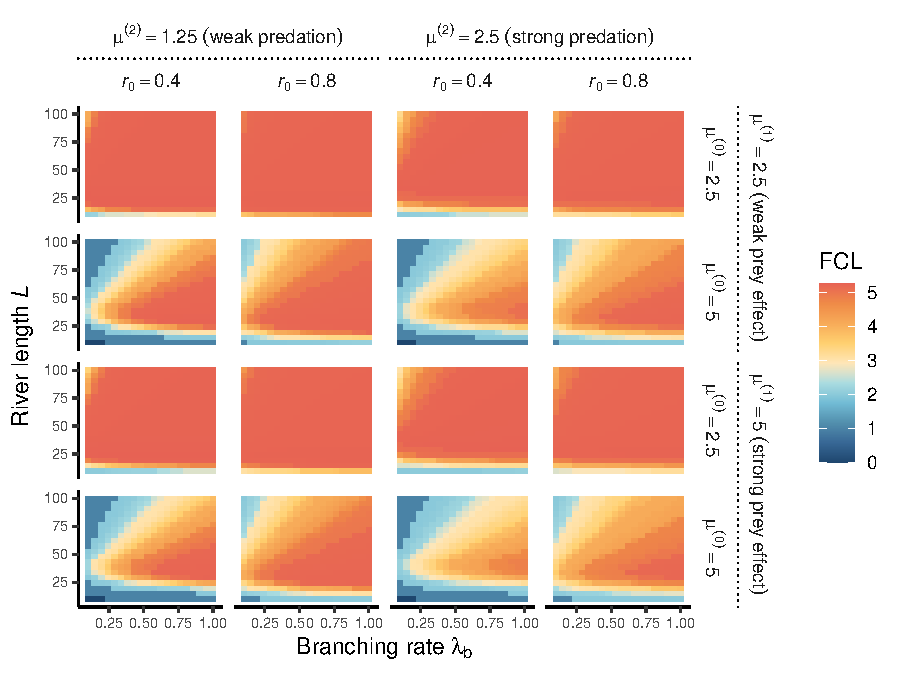
\includegraphics{../output/fig_theo_rho025_g150_theta025.pdf}
\caption{\label{fig:fig-num2}Numerical prediction with high propagule
\(g_0 = 150\), low synchrony \(\rho = 0.25\), and weak omnivory
\(\theta = 0.25\). Heatmaps of FCL are expressed as a function of
ecosystem size (river length, \(L\)) and complexity (branching rate,
\(\lambda_b\)), with rows and columns displaying different combinations
of resource supply (\(r_0\)), disturbance regime (\(\mu^{(0)}\)), prey
effect (\(\mu^{(1)}\)), and predation effect (\(\mu^{(2)}\)). Each cell
represents the average FCL of five food webs. Additional parameter
values are: habitat density \(h=2.5\), dispersal capability
\(\delta_0=0.5\), and scaling exponent \(\psi=0.5\).}
\end{figure}

\newpage

\begin{figure}
\centering
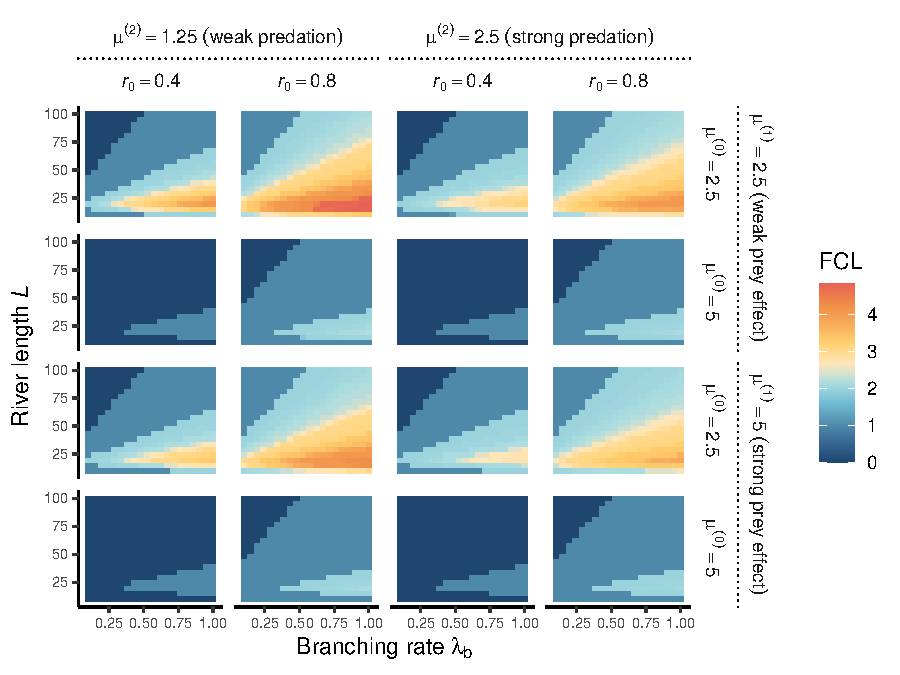
\includegraphics{../output/fig_theo_rho05_g75_theta025.pdf}
\caption{\label{fig:fig-num3}Numerical prediction with low propagule
\(g_0 = 75\), high synchrony \(\rho = 0.5\), and weak omnivory
\(\theta = 0.25\). Heatmaps of FCL are expressed as a function of
ecosystem size (river length, \(L\)) and complexity (branching rate,
\(\lambda_b\)), with rows and columns displaying different combinations
of resource supply (\(r_0\)), disturbance regime (\(\mu^{(0)}\)), prey
effect (\(\mu^{(1)}\)), and predation effect (\(\mu^{(2)}\)). Each cell
represents the average FCL of five food webs. Additional parameter
values are: habitat density \(h=2.5\), dispersal capability
\(\delta_0=0.5\), and scaling exponent \(\psi=0.5\).}
\end{figure}

\newpage

\begin{figure}
\centering
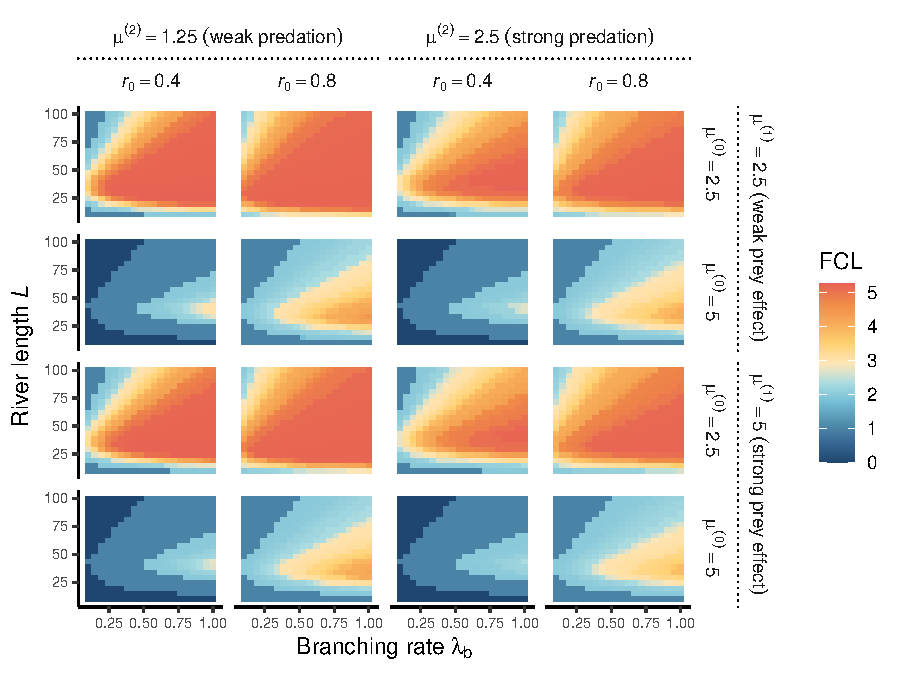
\includegraphics{../output/fig_theo_rho05_g150_theta025.pdf}
\caption{\label{fig:fig-num4}Numerical prediction with high propagule
\(g_0 = 150\), high synchrony \(\rho = 0.5\), and weak omnivory
\(\theta = 0.25\). Heatmaps of FCL are expressed as a function of
ecosystem size (river length, \(L\)) and complexity (branching rate,
\(\lambda_b\)), with rows and columns displaying different combinations
of resource supply (\(r_0\)), disturbance regime (\(\mu^{(0)}\)), prey
effect (\(\mu^{(1)}\)), and predation effect (\(\mu^{(2)}\)). Each cell
represents the average FCL of five food webs. Additional parameter
values are: habitat density \(h=2.5\), dispersal capability
\(\delta_0=0.5\), and scaling exponent \(\psi=0.5\).}
\end{figure}

\newpage

\begin{figure}
\centering
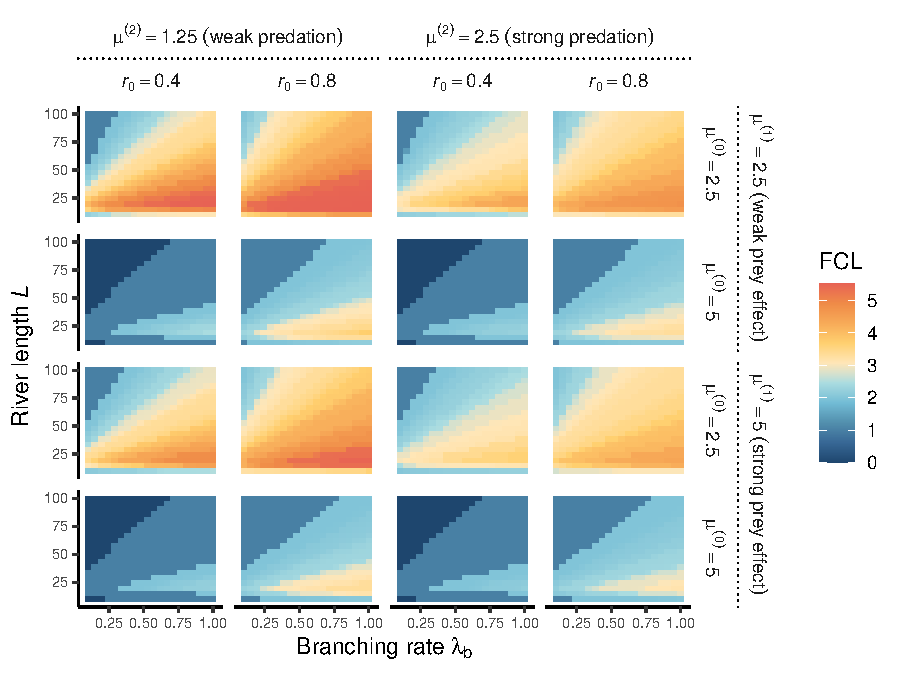
\includegraphics{../output/fig_theo_rho025_g75_theta05.pdf}
\caption{\label{fig:fig-num5}Numerical prediction with low propagule
\(g_0 = 75\), low synchrony \(\rho = 0.25\), and strong omnivory
\(\theta = 0.5\).Heatmaps of FCL are expressed as a function of
ecosystem size (river length, \(L\)) and complexity (branching rate,
\(\lambda_b\)), with rows and columns displaying different combinations
of resource supply (\(r_0\)), disturbance regime (\(\mu^{(0)}\)), prey
effect (\(\mu^{(1)}\)), and predation effect (\(\mu^{(2)}\)). Each cell
represents the average FCL of five food webs. Additional parameter
values are: habitat density \(h=2.5\), dispersal capability
\(\delta_0=0.5\), and scaling exponent \(\psi=0.5\).}
\end{figure}

\newpage

\begin{figure}
\centering
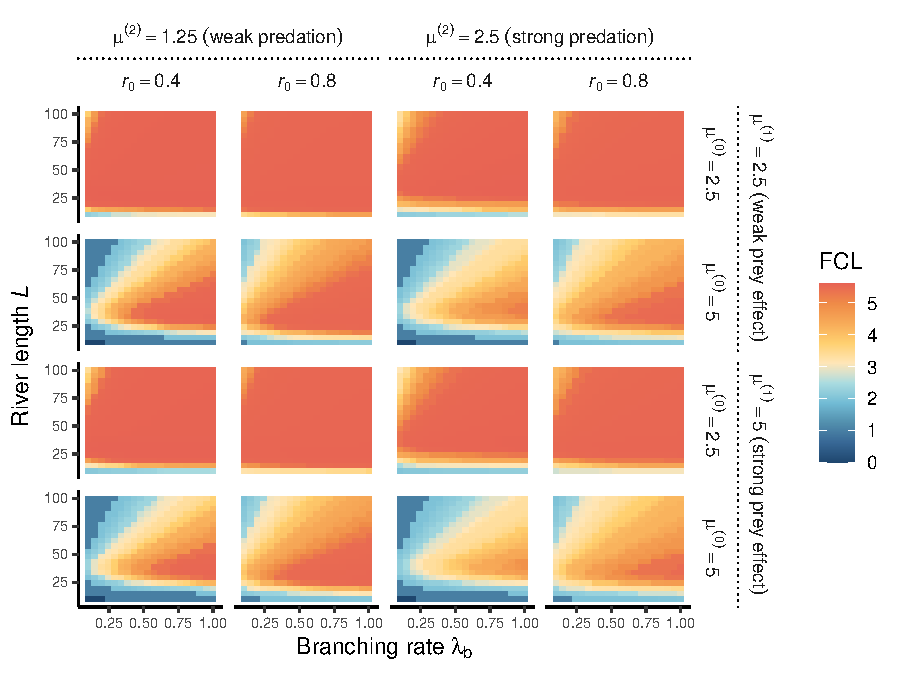
\includegraphics{../output/fig_theo_rho025_g150_theta05.pdf}
\caption{\label{fig:fig-num6}Numerical prediction with high propagule
\(g_0 = 150\), low synchrony \(\rho = 0.25\), and strong omnivory
\(\theta = 0.5\).Heatmaps of FCL are expressed as a function of
ecosystem size (river length, \(L\)) and complexity (branching rate,
\(\lambda_b\)), with rows and columns displaying different combinations
of resource supply (\(r_0\)), disturbance regime (\(\mu^{(0)}\)), prey
effect (\(\mu^{(1)}\)), and predation effect (\(\mu^{(2)}\)). Each cell
represents the average FCL of five food webs. Additional parameter
values are: habitat density \(h=2.5\), dispersal capability
\(\delta_0=0.5\), and scaling exponent \(\psi=0.5\).}
\end{figure}

\newpage

\begin{figure}
\centering
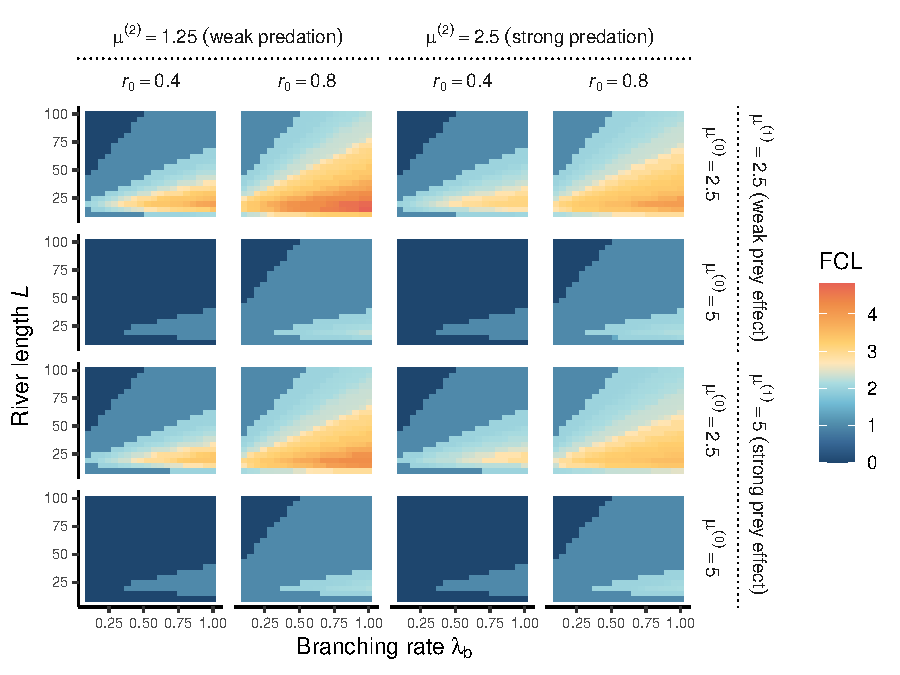
\includegraphics{../output/fig_theo_rho05_g75_theta05.pdf}
\caption{\label{fig:fig-num7}Numerical prediction with low propagule
\(g_0 = 75\), high synchrony \(\rho = 0.5\), and strong omnivory
\(\theta = 0.5\).Heatmaps of FCL are expressed as a function of
ecosystem size (river length, \(L\)) and complexity (branching rate,
\(\lambda_b\)), with rows and columns displaying different combinations
of resource supply (\(r_0\)), disturbance regime (\(\mu^{(0)}\)), prey
effect (\(\mu^{(1)}\)), and predation effect (\(\mu^{(2)}\)). Each cell
represents the average FCL of five food webs. Additional parameter
values are: habitat density \(h=2.5\), dispersal capability
\(\delta_0=0.5\), and scaling exponent \(\psi=0.5\).}
\end{figure}

\newpage

\begin{figure}
\centering
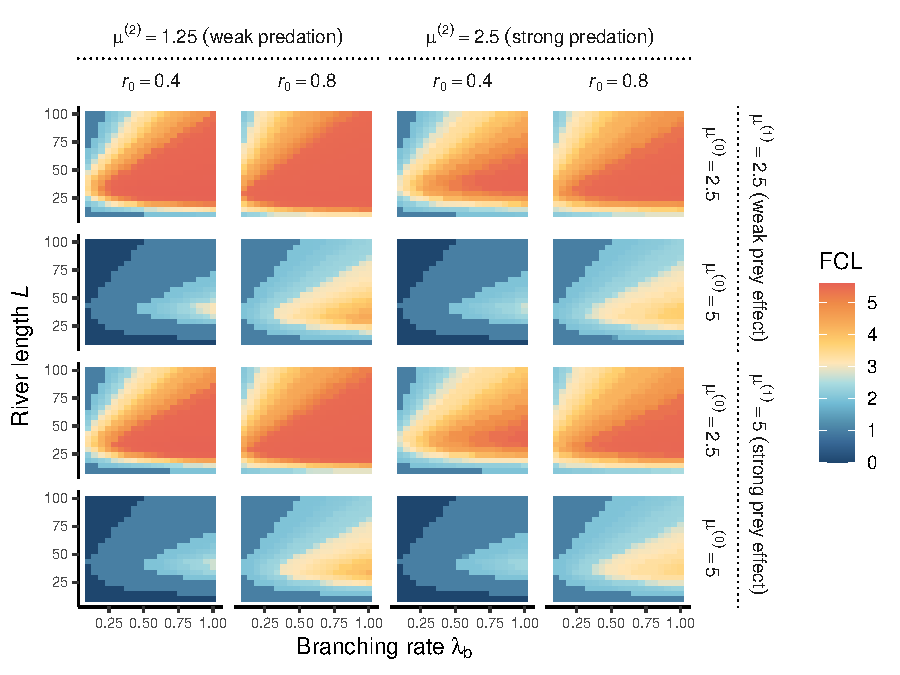
\includegraphics{../output/fig_theo_rho05_g150_theta05.pdf}
\caption{\label{fig:fig-num8}Numerical prediction with high propagule
\(g_0 = 150\), high synchrony \(\rho = 0.5\), and strong omnivory
\(\theta = 0.5\).Heatmaps of FCL are expressed as a function of
ecosystem size (river length, \(L\)) and complexity (branching rate,
\(\lambda_b\)), with rows and columns displaying different combinations
of resource supply (\(r_0\)), disturbance regime (\(\mu^{(0)}\)), prey
effect (\(\mu^{(1)}\)), and predation effect (\(\mu^{(2)}\)). Each cell
represents the average FCL of five food webs. Additional parameter
values are: habitat density \(h=2.5\), dispersal capability
\(\delta_0=0.5\), and scaling exponent \(\psi=0.5\).}
\end{figure}

\newpage


\section{Empirical Analysis}

\subsection{Data Sources}

Table \ref{tab:meta-list} lists 46 studies that were used in our empirical analysis.
These studies contained at least one site that (i) contains either stable isotope data of nitrogen ($\delta^{15}N$) for top and baseline species (primary producer or consumer) or an estimate of the maximum trophic position; (ii) contains reliable spatial coordinates for geospatial analysis; (iii) is located within a freshwater lotic system, excluding lentic (reservoirs, wetlands, lakes) and semi-lentic systems (large rivers with $>$ 5000 km$^2$ in watershed area); (iv) can be associated with potential environmental drivers in GIS.
When multiple estimates of FCL were available (e.g., from inter-annual or seasonal replicates), we averaged these values so that each site was represented by a single FCL estimate.

To evaluate coordinate precision, we classified data into the following categories:

\begin{itemize}
    \item Category \textbf{1}: Exact coordinates available, either provided directly in the article or obtained through author correspondence.
    \item Category \textbf{2}: Near-exact coordinates identified from text descriptions.
    \item Category \textbf{3}: Coordinates visually inferred from a map, using reference landmarks or river geomorphology.
    \item Category \textbf{4}: Coordinates estimated based on river name or by aggregating multiple sites.
    \item Category \textbf{5}: Coordinates unavailable.
\end{itemize}

Categories \textbf{4} and \textbf{5} were excluded from our analysis.

\begingroup\small
\begin{longtable}{p{0.1\textwidth}p{0.9\textwidth}}
\caption{List of publications included in the meta-analysis.
             `Code' refers to the unique identifier assigned to each study for use in the analysis.} \\ 
  \hline
Code & Publication \\ 
  \hline
001 & Wilkinson, C.L. \textit{et al}. 2021 Forest conversion to oil palm compresses food chain length in tropical streams. \textit{Ecology} 102: e03199 \\ 
  003 & Jackson, M.C. \textit{et al}. 2020 Food web properties vary with climate and land use in South African streams. \textit{Functional Ecology} 34: 1653-1665 \\ 
  004 & Sroczynska, K. \textit{et al}. 2020 Food web structure of three Mediterranean stream reaches along a gradient of anthropogenic impact. \textit{Hydrobiologia} 847: 2357-2375 \\ 
  007 & Kelson, S.J. \textit{et al}. 2020 Partial migration alters population ecology and food chain length: evidence from a salmonid fish. \textit{Ecosphere} 11: e03044 \\ 
  008 & Boddy, N.C. \textit{et al}. 2020 Big impacts from small abstractions: The effects of surface water abstraction on freshwater fish assemblages. \textit{Aquatic Conservation: Marine and Freshwater Ecosystems} 30: 159-172 \\ 
  009 & Pearce, J.L. \textit{et al}. 2019 Unrestricted ramping rates and long-term trends in the food web metrics of a boreal river. \textit{River Research and Applications} 35: 1575-1589 \\ 
  010 & Negishi, J.N. \textit{et al}. 2019 High resilience of aquatic community to a 100-year flood in a gravel-bed river. \textit{Landscape and Ecological Engineering} 15: 143-154 \\ 
  011 & Pease, A.A. \textit{et al}. 2019 Trophic structure of fish assemblages varies across a Mesoamerican river network with contrasting climate and flow conditions. \textit{Food Webs} 18: e00113 \\ 
  013 & Sullivan, S.M.P. \textit{et al}. 2019 Artificial lighting at night alters aquatic-riparian invertebrate food webs. \textit{Ecological Applications} 29: e01821 \\ 
  014 & Fraley, K.M. \textit{et al}. 2018 Responsiveness of fish mass-abundance relationships and trophic metrics to flood disturbance, stream size, land cover and predator taxa presence in headwater streams. \textit{Ecology of Freshwater Fish} 27: 999-1014 \\ 
  018 & Gonzalez-Bergonzoni, I. \textit{et al}. 2018 Riparian forest modifies fuelling sources for stream food webs but not food-chain length in lowland streams of Denmark. \textit{Hydrobiologia} 805: 291-310 \\ 
  019 & Kaymak, N. \textit{et al}. 2018 Spatial and temporal variation in food web structure of an impounded river in Anatolia. \textit{Marine and Freshwater Research} 69: 1453-1471 \\ 
  020 & Ceneviva-Bastos, M. \textit{et al}. 2017 Responses of aquatic food webs to the addition of structural complexity and basal resource diversity in degraded Neotropical streams. \textit{Austral Ecology} 42: 908-919 \\ 
  021 & Taylor, G.C. \textit{et al}. 2017 Comparing the fish assemblages and food-web structures of large floodplain rivers. \textit{Freshwater Biology} 62: 1891-1907 \\ 
  023 & Majdi, N. and Traunspurger, W. 2017 Leaf fall affects the isotopic niches of meiofauna and macrofauna in a stream food web. \textit{Food Webs} 10: 5-14 \\ 
  025 & Kautza, A. and Sullivan, S.M.P. 2016 Anthropogenic and natural determinants of fish food-chain length in a midsize river system. \textit{Freshwater Science} 35: 895-908 \\ 
  026 & Ruhi, A. \textit{et al}. 2016 Flow regulation increases food-chain length through omnivory mechanisms in a Mediterranean river network. \textit{Freshwater Biology} 61: 1536-1549 \\ 
  028 & Jardine, T.D. 2016 A top predator forages low on species-rich tropical food chains. \textit{Freshwater Science} 35: 666-675 \\ 
  033 & Hette-Tronquart, N. \textit{et al}. 2013 Variability of water temperature may influence food-chain length in temperate streams. \textit{Hydrobiologia} 718: 159-172 \\ 
  037 & Riva-Murray, K. \textit{et al}. 2011 Spatial patterns of mercury in macroinvertebrates and fishes from streams of two contrasting forested landscapes in the eastern United States. \textit{Ecotoxicology} 20: 1530-1542 \\ 
  039 & Pilger, T. J. \textit{et al}. 2010 Diet and trophic niche overlap of native and nonnative fishes in the Gila River, USA: Implications for native fish conservation. \textit{Ecology of Freshwater Fish} 19: 300-321 \\ 
  044 & Singer, G.A. and Battin, T.J. 2007 Anthropogenic subsidies alter stream consumer-resource stoichiometry, biodiversity, and food chains. \textit{Ecological Applications} 17: 376-389 \\ 
  048 & Orr, P.L. \textit{et al}. 2006 Food chain transfer of selenium in lentic and lotic habitats of a western Canadian watershed. \textit{Ecotoxicology and Environmental Safety} 63: 175-188 \\ 
  052 & Lake, J.L. \textit{et al}. 2001 Stable nitrogen isotopes as indicators of anthropogenic activities in small freshwater systems. \textit{Canadian Journal of Fisheries and Aquatic Sciences} 58: 870-878 \\ 
  055 & Angradi T.R. 1994 Trophic linkages in the lower Colorado River: Multiple stable isotope evidence. \textit{Journal of the North American Benthological Society} 13: 479-495 \\ 
  065 & Bunn, S.E. \textit{et al}. 1997 Contributions of sugar cane and invasive pasture grass to the aquatic food web of a tropical lowland stream. \textit{Marine and Freshwater Research} 48: 173-179 \\ 
  068 & Perry, R.W. \textit{et al}. 2003 Effects of disturbance on contribution of energy sources to growth of juvenile chinook salmon (Oncorhynchus tshawytscha) in boreal streams. \textit{Canadian Journal of Fisheries and Aquatic Sciences} 60: 390-400 \\ 
  072 & Doucett, R.R. \textit{et al}. 1996 Stable isotope analysis of nutrient pathways leading to Atlantic salmon. \textit{Canadian Journal of Fisheries and Aquatic Sciences} 53: 2058-2066 \\ 
  073 & Charles, K. \textit{et al}. 2004 Estimating the contribution of sympatric anadromous and freshwater resident brown trout to juvenile production. \textit{Marine and Freshwater Research} 55: 185-191 \\ 
  074 & March, J.G. and Pringle, C.M. 2003 Food web structure and basal resource utilization along a tropical island stream continuum, Puerto Rico. \textit{Biotropica} 35: 84-93 \\ 
  075 & Steffy, L. and Kilham, S.S. 2004 Elevated delta N-15 in stream biota in areas with septic tank systems in an urban watershed.. \textit{Ecological Applications} 14: 637-641 \\ 
  078 & Sabo, J. L. \textit{et al}. 2010 The role of discharge variation in scaling of drainage area and food chain length in rivers. \textit{Science} 330: 965-967 \\ 
  080 & Itakura, H. \textit{et al}. 2020 Anguillid eels as a surrogate species for conservation of freshwater biodiversity in Japan. \textit{Scientific Reports} 10: 8790 \\ 
  081 & Burdon, F.J. \textit{et al}. 2020 Mechanisms of trophic niche compression: Evidence from landscape disturbance. \textit{Journal of Animal Ecology} 89: 730-744 \\ 
  082 & Fraley, K.M. \textit{et al}. 2020 Influence of maternally-transferred nitrogen and carbon on stable isotope ratios in juvenile chinook salmon. \textit{North American Journal of Fisheries Management} 40: 175-181 \\ 
  083 & Maitland, B.M. and Rahel, F.J. 2023 Aquatic food web expansion and trophic redundancy along the Rocky Mountain–Great Plains ecotone. \textit{Ecology} 104: e4103 \\ 
  089 & Dekar, M.P. \textit{et al}. 2009 Shifts in the trophic base of intermittent stream food webs. \textit{Hydrobiologia} 635: 263-277 \\ 
  091 & Doi, H. \textit{et al}. 2006 Contribution of chemoautotrophic production to freshwater macroinvertebrates in a headwater stream using multiple stable isotopes. \textit{International Review of Hydrobiology} 91: 501-508 \\ 
  098 & Hoeinghaus, D.J. \textit{et al}. 2008 Hydrogeomorphology and river impoundment affect food-chain length of diverse Neotropical food webs. \textit{Oikos} 117: 984-995 \\ 
  099 & Huang, I.Y. \textit{et al}. 2007 Food web structure of a subtropical headwater stream. \textit{Marine and Freshwater Research} 58: 596-607 \\ 
  101 & Jepsen, D.B. and Winemiller, K.O. 2007 Basin geochemistry and isotopic ratios of fishes and basal production sources in four neotropical rivers. \textit{Ecology of Freshwater Fish} 16: 267-281 \\ 
  108 & Mercado‐Silva, N. \textit{et al}. 2009 The effects of impoundment and non-native species on a river food web in Mexico's central plateau. \textit{River Research and Applications} 25: 1090-1108 \\ 
  110 & Reid, D.J. \textit{et al}. 2008 Terrestrial detritus supports the food webs in lowland intermittent streams of south-eastern Australia: a stable isotope study. \textit{Freshwater Biology} 53: 2036-2050 \\ 
  116 & Takamura, K. 2009 Population structuring by weirs and the effect on trophic position of a freshwater fish Zacco platypus in the middle reaches of Japanese rivers. \textit{Fundamental and Applied Limnology} 174: 307-315 \\ 
  117 & Ulseth, A.J. and Hershey, A.E 2005 Natural abundances of stable isotopes trace anthropogenic N and C in an urban stream. \textit{Journal of the North American Benthological Society} 24: 270-289 \\ 
  121 & Winemiller, K.O. \textit{et al}. 2011 Stable isotope analysis reveals food web structure and watershed impacts along the fluvial gradient of a Mesoamerican coastal river. \textit{River Research and Applications} 27: 791-803 \\ 
   \hline
\hline
\label{tab:meta-list}
\end{longtable}
\endgroup


\subsection{Parameter Estimate}

Table \ref{tab:parms-est} presents the parameter estimates of the random-intercept model detailed in the main text.
The 95\% credible intervals and posterior probabilities are estimated based on 2,000 posterior MCMC samples.

\begin{table}[ht]
\centering
\caption{Parameter estimates of the hierarchical Bayesian model 
             with corresponding 95\% credible intervals (CIs) and 
             posterior probabilities ($\Pr(\cdot)$), 
             representing the uncertainty around each parameter estimate.
             \label{tab:parms-est}} 
\begingroup\small
\begin{tabularx}{\textwidth}{llllll}
  \hline
Symbol & Description & Estimate & 95\% CI & $\Pr(< 0)$ & $\Pr(> 0)$ \\ 
  \hline
$\alpha_1$ & Elevation & $-0.03$ & [$-0.06$, $0.00$] & $0.96$ & $0.04$ \\ 
  $\beta_0$ & Intercept & $1.28$ & [$1.10$, $1.49$] & $0.00$ & $1.00$ \\ 
  $\beta_1$ & ln Total river length & $0.01$ & [$-0.02$, $0.05$] & $0.29$ & $0.71$ \\ 
  $\beta_2$ & ln Branching rate & $0.03$ & [$-0.00$, $0.06$] & $0.05$ & $0.95$ \\ 
  $\beta_3$ & Air temperature & $0.02$ & [$-0.03$, $0.07$] & $0.25$ & $0.75$ \\ 
  $\beta_4$ & Precipitation & $-0.11$ & [$-0.16$, $-0.06$] & $1.00$ & $0.00$ \\ 
  $\beta_5$ & Human footprint & $-0.01$ & [$-0.05$, $0.03$] & $0.74$ & $0.26$ \\ 
  $\nu$ & Degrees of freedom & $4.50$ & [$2.52$, $11.16$] & $0.00$ & $1.00$ \\ 
  $\sigma$ & Site-level residual SD & $0.09$ & [$0.07$, $0.12$] & $0.00$ & $1.00$ \\ 
  $\sigma_{\varepsilon}$ & Watershed-level SD (random effect) & $0.06$ & [$0.02$, $0.11$] & $0.00$ & $1.00$ \\ 
  $\sigma_{\eta}$ & Region-level SD (random effect) & $0.19$ & [$0.09$, $0.55$] & $0.00$ & $1.00$ \\ 
  $\xi_{1}$ & Scaling exponent for the number of sites & $0.18$ & [$0.01$, $0.70$] & $0.00$ & $1.00$ \\ 
  $\xi_{2}$ & Scaling parameter for spatial sampling randomness & $0.86$ & [$0.05$, $2.65$] & $0.00$ & $1.00$ \\ 
   \hline
\end{tabularx}
\endgroup
\end{table}


\subsection{Discharge-Precipitation Relationship}
We used daily river discharge data from 2000 to 2015, simulated by the Global Hydrodynamics model \textit{CaMa-Flood}, to estimate flow variability  \citep{yamazaki_deriving_2009, kimura_methodology_2023, lin_global_2019}.
The discharge data is available at a 0.1-degree resolution (approximately 10 km at the equator) and was extracted from the nearest flow-connected cell for each site; however, discharge data could not be obtained for two headwater stream sites, which were excluded from further analysis.
At each site, we log-transformed the discharge data and then scaled it by the temporal mean to facilitate comparison across sites with varying stream sizes.

We define ``flow variability'' as the magnitude of discharge deviations from seasonal expectations.
To model this variability, we fitted a Generalized Additive Model (GAM) as follows:

\begin{align}
    \begin{split}
    D_i &= \alpha_d + s(\mbox{Julian}_i) + \varepsilon_i,\\
    \varepsilon_i &\sim t(0, \sigma_d^2, \nu_d),
    \end{split}
\end{align}

where $D_i$ represents the scaled daily discharge, ``$\mbox{Julian}_i$'' refers to the Julian date (with the first day of the year as the origin), and $s(\cdot)$ denotes the smoothing function.
We used a Student's t-distribution for the error structure, as it better captures the fat-tailed nature of the discharge data.
The degree of freedom, $\nu_d$, characterizes the thickness of the tails, with smaller values indicating a higher likelihood of extreme high or low flows relative to seasonal expectations (i.e., fatter tails).
As $\nu_d$ approaches infinity, the Student's t-distribution converges to a normal distribution.

We regressed the log-transformed degrees of freedom ($\ln \nu_d$) on the log-transformed regional precipitation (i.e., the watershed average; see Methods) using a linear mixed-effects model with random effects for watershed ID and hydrological region.
The model revealed a significant negative scaling relationship, described by the equation $\ln \nu_d = 16.84 - 2.02 \cdot \ln \text{precipitation} + \text{error}$ (SE for intercept: 4.01, SE for slope: 0.57).
This result suggests that watersheds with higher precipitation are more likely to experience extreme high or low flows relative to seasonal norms.

\subsection{Distance Ratio}

The distance ratio, $d_{w}$, was used to evaluate the randomness of the spatial sampling design within watershed $w$.
The procedure consists of the following steps:

\begin{enumerate}
    \item Dummy sites were randomly generated along the river network. The number of dummy sites matched the number of actual sampling sites in the observations.
    \item Euclidean distance for each pair of sites was calculated, and the median distance was determined.
    \item Steps 1 and 2 were repeated 100 times to compute the average of the median distances, denoted as $\mu_d$.
    \item Finally, $d_{w}$ was calculated as the ratio of the observed median distance to $\mu_d$.
\end{enumerate}

Therefore, the distance ratio $d_{w}$ represents the spatial randomness of actual sampling sites, with values smaller (greater) than one indicating over-aggregation (over-dispersion) of sampling sites.
We assumed $d_{w} = 0$ if there was only one site within a watershed.

\subsection{Competing Model}

The hierarchical model presented in the main text is a random intercept model, which assumes no geographic variation in the effects of river length and branching rate. To allow for geographic variation, we developed a random intercept-slope model, where the effects of river length and branching rate vary by geographic region $u$.

Specifically, we modified the watershed-level regression equation as follows:

\begin{equation}
    \alpha_{0, w} = \beta_{0, u[w]} + \beta_{1, u[w]} L_w + \beta_{2, u[w]} \lambda_{b, w} + \sum_m \beta_m x'_{m, w} + \varepsilon_{w},
    \label{eq:watershed-average}
\end{equation}

and

\begin{equation}
    \boldsymbol{\beta_u} \sim \mbox{MVN}(\boldsymbol{\mu_{\beta}}, \Omega),
\end{equation}

where $\boldsymbol{\beta_u} = \{\beta_{0, u}, \beta_{1, u}, \beta_{2, u}\}$. Here, $\boldsymbol{\mu_{\beta}}$ represents the mean vector, and $\Omega$ denotes the variance-covariance matrix.
We used weakly informative priors, where $\boldsymbol{\mu_{\beta}} \sim \mbox{Normal}(0, 5^2)$, $U_{\Omega} \sim \mbox{LkjCholesky}(2.0)$, and $\sigma_{\beta, m} \sim t^+(0, 1, 10)$ ($m \in \{0, 1, 2\}$). In this context, the upper-triangular matrix $U_{\Omega}$ is the Cholesky factor for the correlation matrix, and $\sigma_{\beta, m}$ represents the standard deviations in $\Omega$.
Other priors were specified as described in the main text.

Four Markov chain Monte Carlo (MCMC) chains were run until parameter estimates
converged.
The total number of MCMC iterations per chain was 60,000, in which MCMC samples were saved every 60 steps after the initial 30,000 burn-in period.
As a result, we used a total of $500 \times 4 = 2,000$ MCMC samples for the estimation of posterior distributions.
Convergence was assessed by examining whether the R-hat indicator of each parameter approached < 1.1.

\newpage

\bibliography{references}

\end{document}